% Layout-only review candidate based on main_individual_final_review.tex.
% Compile with: pdflatex -jobname=DT081A_Lab3_Report_Yacoub_Dawli_LAYOUT_REVIEW main_individual_layout_review.tex
\documentclass[10pt,a4paper]{article}
\usepackage[T1]{fontenc}
\usepackage{lmodern}
\usepackage[margin=16mm]{geometry}
\usepackage{graphicx,amsmath,booktabs,caption,float,listings,titlesec,hyperref,placeins}
\hypersetup{hidelinks,pdftitle={Lab 3 Report — Image Processing},
  pdfauthor={Yacoub Dawli}}
\graphicspath{{../figures/}}
\linespread{0.96}
\setlength{\parindent}{0pt}
\setlength{\parskip}{1pt}
\setlength{\intextsep}{3pt}
\setlength{\textfloatsep}{5pt}
\titleformat{\section}{\large\bfseries}{\thesection}{0.6em}{}
\titleformat{\subsection}{\normalsize\bfseries}{\thesubsection}{0.6em}{}
\titlespacing*{\section}{0pt}{4pt}{2pt}
\titlespacing*{\subsection}{0pt}{4pt}{2pt}
\captionsetup{font=normalsize,labelfont=bf,skip=2pt,hypcap=false}
\lstset{basicstyle=\ttfamily\fontsize{8.5}{10}\selectfont,
  columns=fullflexible,keepspaces=true,showstringspaces=false,
  breaklines=true,breakatwhitespace=true,breakindent=8pt,
  postbreak=\mbox{$\hookrightarrow$\space},
  aboveskip=1pt,belowskip=2pt}
\setlength{\emergencystretch}{1em}
\clubpenalty=10000
\widowpenalty=10000
\raggedbottom
\renewcommand{\topfraction}{0.9}
\renewcommand{\bottomfraction}{0.9}
\renewcommand{\textfraction}{0.08}
\renewcommand{\floatpagefraction}{0.75}
\pagestyle{plain}

\begin{document}
\begin{center}
{\large DT081A - Signal and Image Processing}\\[2pt]
{\large\bfseries Lab 3 Report --- Image Processing}\\[3pt]
Yacoub Dawli --- \texttt{yada2100@student.miun.se}\\[2pt]
{\small 24 October 2026}
\end{center}
\vspace{-5pt}

\section{Introduction}
This lab covered pixel transforms, colour reduction, filtering, Fourier analysis,
histograms and morphology, comparing image changes, time and memory use.

\section{Experimental Setup}
The experiments used Python, NumPy, OpenCV and Matplotlib, with the \(512\times512\) \texttt{peppers.tiff} test image. BGR was converted to RGB for display, with grayscale and synthetic images used where needed.

\section{Results and Analysis}
\subsection{Gamma Correction}
\textbf{Q1.1.} The formula \(255(I/255)^\gamma\), at \(\gamma=2.0\), darkened the three inputs
(Table~\ref{tab:gamma}); \texttt{uint8} drops fractional parts.

\begin{table}[H]
\centering
\caption{Gamma calculation, \(\gamma=2.0\).}\label{tab:gamma}
\begin{tabular}{rrr}\toprule
Input & Before integer conversion & \texttt{uint8} output\\\midrule
64 & 16.063 & 16\\
128 & 64.251 & 64\\
192 & 144.565 & 144\\\bottomrule
\end{tabular}
\end{table}

\textbf{Q1.2.} At \(\gamma=2.2\), mean intensity fell from 120.22 to 61.00.
The image darkened; its histogram moved lower, with integer-conversion gaps
(Figure~\ref{fig:gamma}). This relates to unequal visual sensitivity, but is not
an exact logarithmic eye model. The lab uses \(\gamma\), not camera pre-correction's \(1/\gamma\).



\begin{figure}[!htbp]\centering
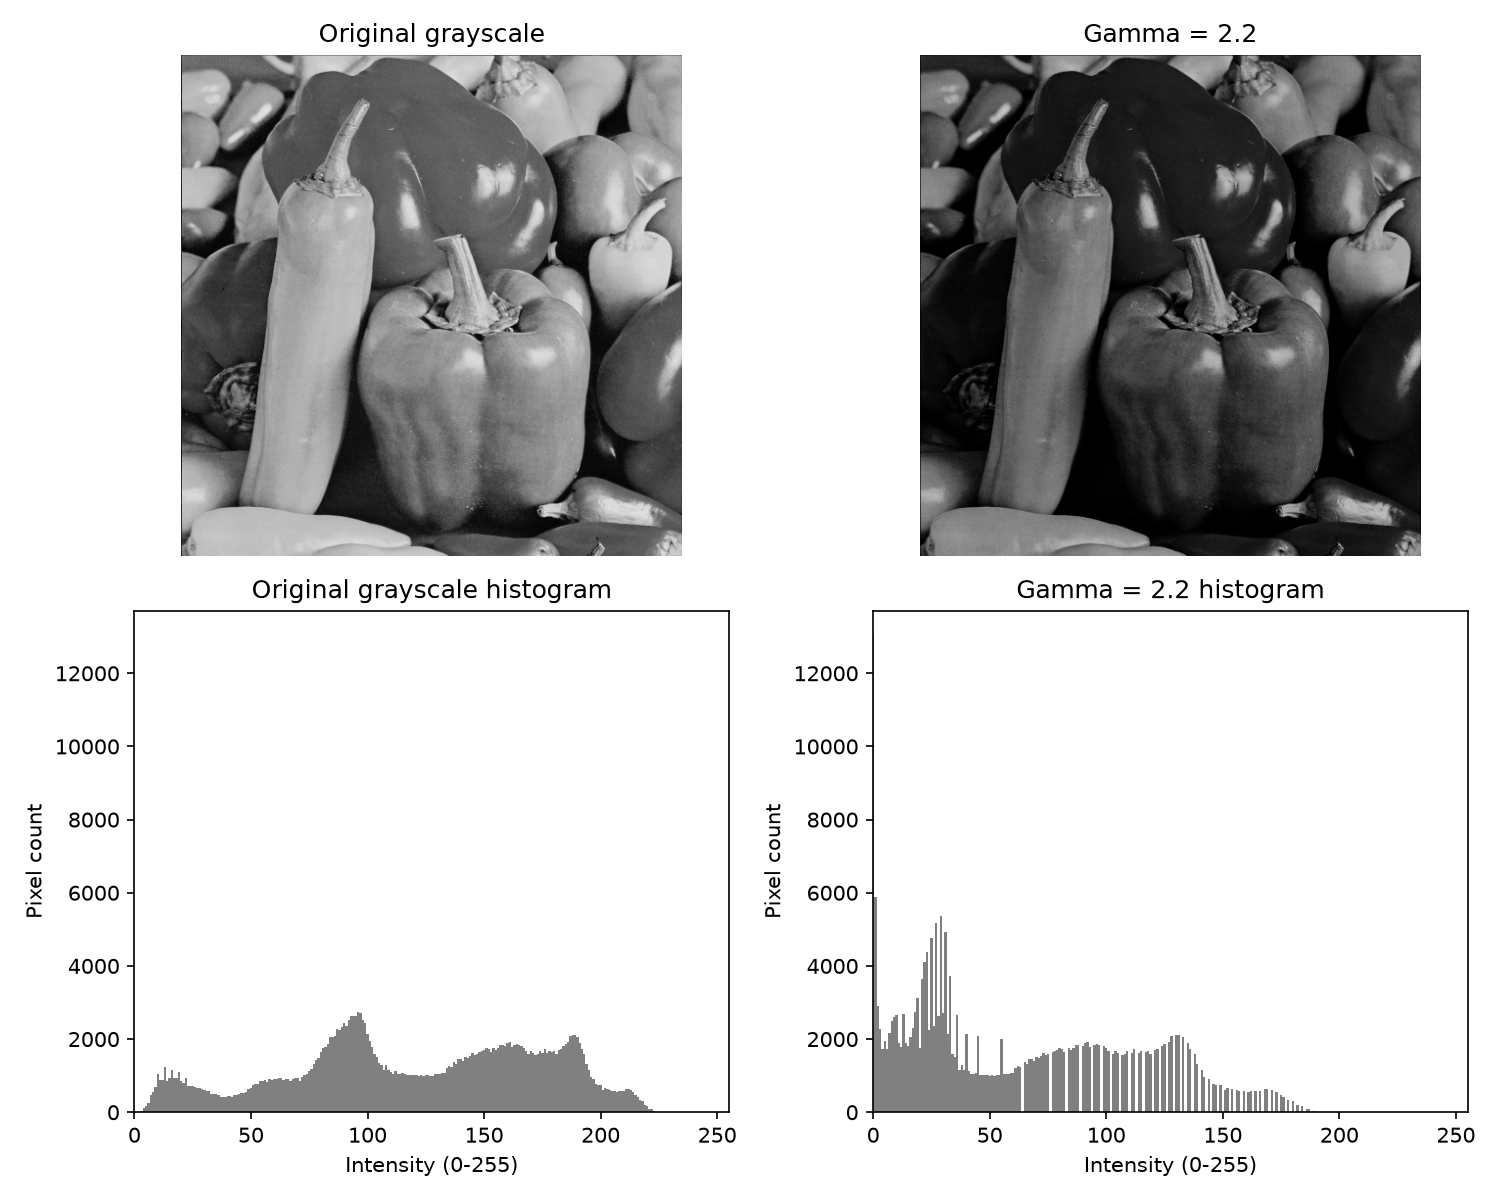
\includegraphics[trim=0 0 0 273.6bp,clip,width=160mm]{section1_gamma_histograms.png}
\caption{Q1.2: original and gamma-2.2 histograms from the same experiment.}\label{fig:gamma}
\end{figure}

\subsection{Colorspaces}
\textbf{Q2.1.} OpenCV orders channels Y, Cr, Cb; \(Y\approx0.299R+0.587G+0.114B\).
All minima were 0; Y/R/G/B maxima were 228/231/237/229 and standard deviations
53.88/45.17/75.05/44.29. G was widest, then Y; R had many high values, B mostly low.
Y gives one brightness channel for edge detection, but can miss equal-brightness colour boundaries.

\textbf{Q2.2.} Y stayed unchanged; both chroma dimensions were reduced by factors 2, 4 and 8,
using area reduction and linear reconstruction. Factor 2 gives
\(3N\to N+N/4+N/4=1.5N\): 786,432 to 393,216 bytes, saving 50\%.
Factors 4/8 need 294,912/270,336 bytes, saving 62.5/65.625\% before reconstruction,
not compressed files. Factor 2 looked close; 4 softened colour boundaries;
8 blended colours more, while Y detail remained.

\subsection{Quantization and Sampling}
\textbf{Q3.1.} RGB integer division by 16 gave 16 possible levels, displayed as
\(0,16,\ldots,240\). Only 15 were used: no input reached 240. Colours became
stepped and darker. Packed 4-bit storage gives \(2{:}1\), or 50\% saving:
393,216 versus 786,432 bytes. The actual \texttt{uint8} array stayed at 786,432 bytes.

\textbf{Q3.2.} Grayscale division by 32 groups 32 intensities into each of eight levels
\(0,32,\ldots,224\). All eight were used; the last held 29 pixels.
Both histograms count 262,144 pixels (Figure~\ref{fig:3bit}). Grouping caused banding
and lost shading/texture, although outlines remained.



\begin{figure}[!htbp]\centering
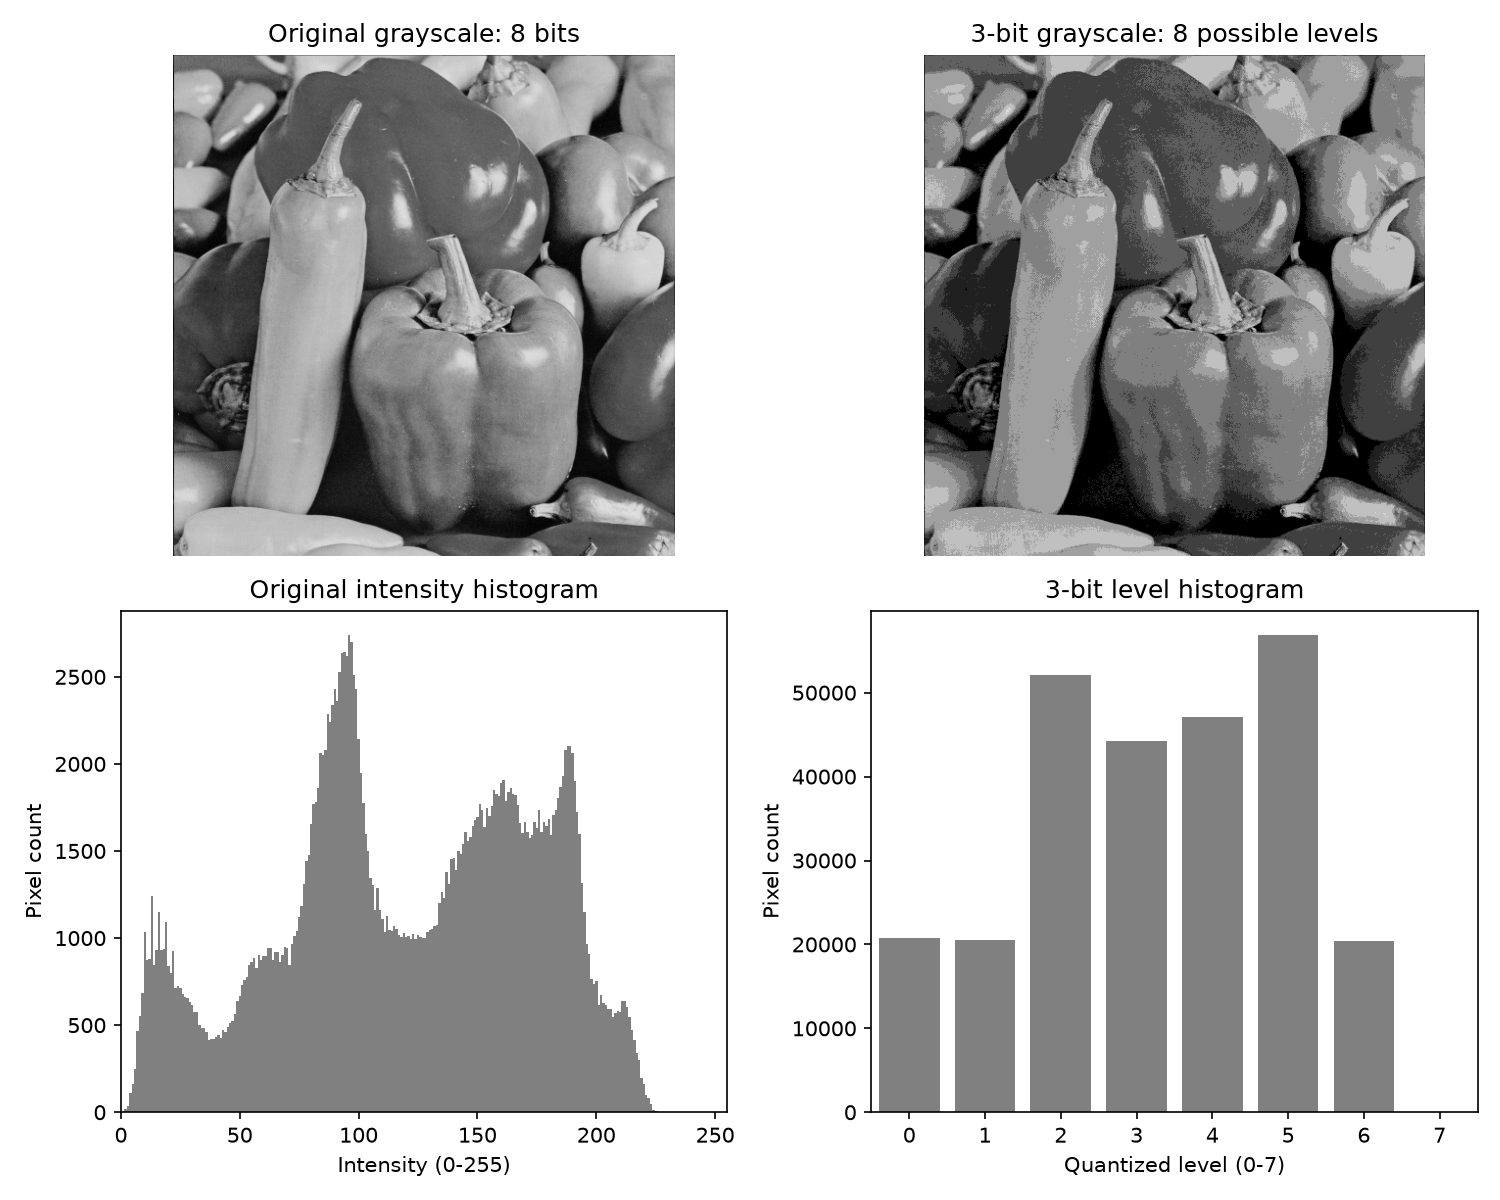
\includegraphics[trim=0 0 0 273.6bp,clip,width=160mm]{section3_3bit_histograms.png}
\caption{Q3.2: original and 3-bit histograms; count scales are labelled separately.}\label{fig:3bit}
\end{figure}

\subsection{Convolution and Edge Detection}
\textbf{Q4.1.} Matching \(\sigma=1\) Gaussian kernels used float64 and
\texttt{BORDER\_REFLECT\_101}, after warm-up (30 runs). Recorded 2D/separable means in ms were: \(5\times5\): 5.420/1.429; \(11\times11\): 9.880/10.455; \(21\times21\): 23.481/24.022. Loading and plotting were excluded. Separable was
faster only at \(5\times5\); 2D was slightly faster at 11 and 21. Reducing
\(k^2\) weights to about \(2k\) can help large kernels, but library routines affect
speed. Outputs looked alike, differing by at most about 0.000002 intensity units.



\textbf{Q4.2.} The \(3\times3\) Sobel function used \texttt{dx=0, dy=1}.
Absolute top-to-bottom changes highlighted horizontal boundaries and weakened
vertical sides. With \texttt{dx=1, dy=0}, vertical edges stood out; curves appeared in both.

\textbf{Q4.3.} Signed derivatives gave \(G=\sqrt{G_x^2+G_y^2}\), with a copy normalized
to 0--255. Combining directions completed outlines/stems; brighter means stronger
edges (Figure~\ref{fig:gradients}, right).

\subsection{Matrix Operations}
\textbf{Q5.1.} Stacking, applying \(1.2(I-128)+128+20\), clipping to 0--255 and reshaping
gave identical brighter NumPy/loop images, with clipped highlights. NumPy was
229.82 times faster using unrounded times (NumPy 2.040 ms; loops 468.915 ms, 5 runs), avoiding Python
operations per pixel. Timing included calculation, output creation and conversion.

\textbf{Q5.2.} The 262,144-value vector gives H \(262{,}144^2=68{,}719{,}476{,}736\)
elements. Float32 needs 274,877,906,944 bytes (256 GiB); float64
549,755,813,888 bytes (512 GiB), with GiB = \(1024^3\) bytes. H was not allocated.
Most entries would be zero; storing nine weights and filtering locally is more practical.

\subsection{Pixel-Based Processing}
\begin{minipage}[t]{0.55\linewidth}\vspace{0pt}
\textbf{Q6.1.} Direct and 256-entry lookup outputs were identical \texttt{uint8}, range
0--240. Lookup was 3.84 times faster (direct 9.469 ms; lookup 2.468 ms), reusing logarithms.
Its separate 0.539 ms construction was excluded; warmed-up applications were averaged over 30 calls.

\textbf{Q6.2.} Two log halves joined at 127.5, strength 4 (Figure~\ref{fig:log}).
The middle is steeper, the ends flatter: input gaps 32 gave output gaps
17 (0--32), 64 (112--144), 18 (223--255). Middle shading separated;
shadows/highlights compressed. Dark gaps darkened and light areas brightened.
Intensity order and endpoints 0 and 255 stayed unchanged.
\end{minipage}\hfill
\begin{minipage}[t]{0.43\linewidth}\vspace{0pt}\centering
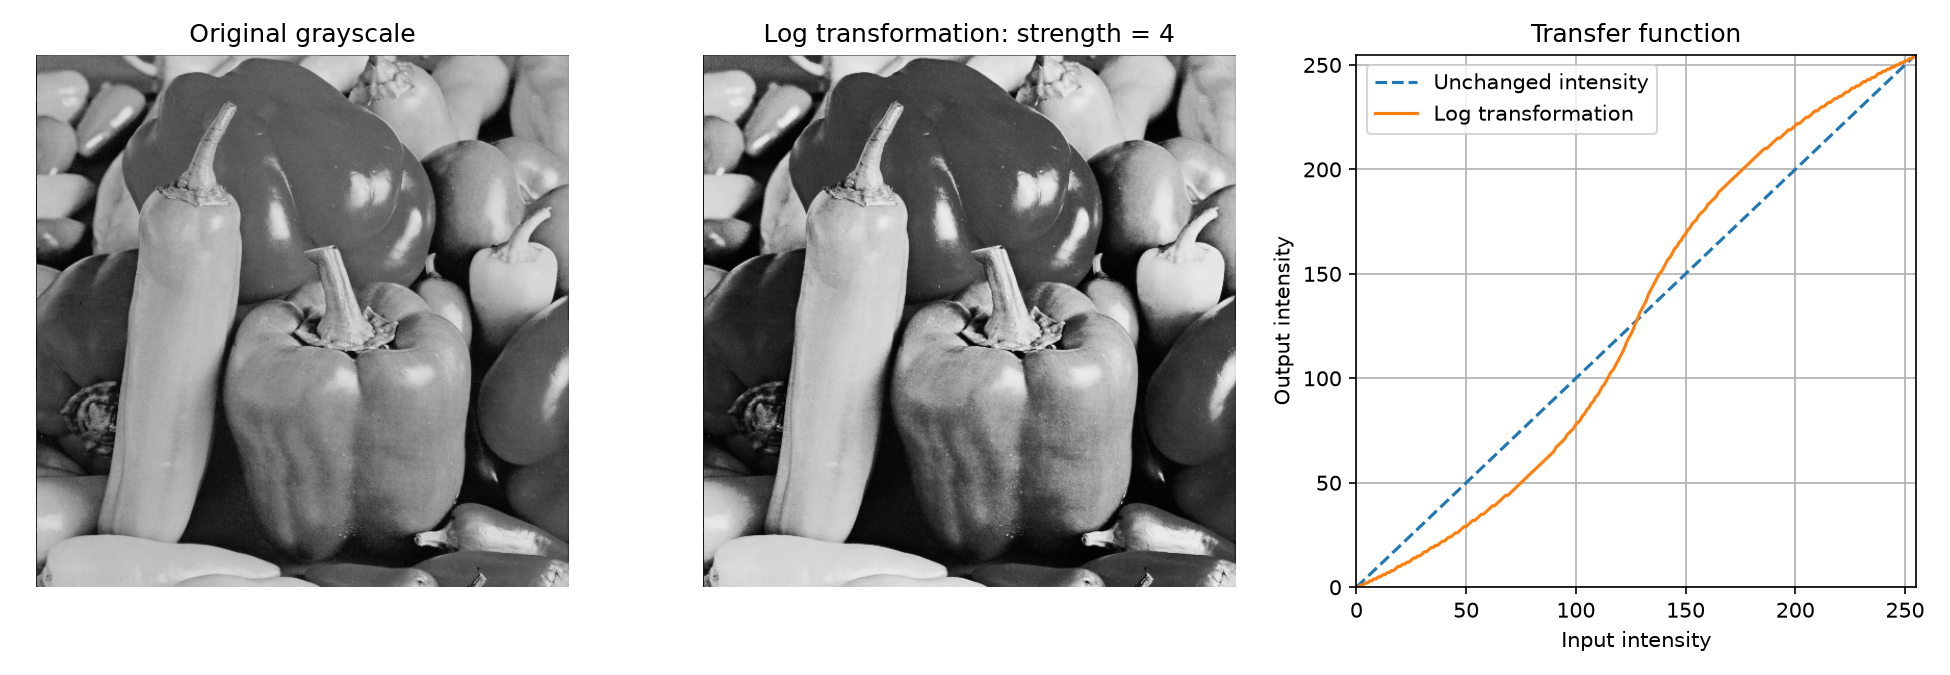
\includegraphics[trim=609.6bp 0 0 0,clip,width=\linewidth]{section6_log_transformation.png}
\captionof{figure}{Q6.2: logarithmic transfer curve; dashed line is unchanged intensity.}\label{fig:log}
\end{minipage}

\subsection{Elementary Images}
\textbf{Q7.1.} The teacher's outer products made \(16\times16\) images:
Ramp\(\times\)Ramp gave two-direction gradients; Step\(\times\)Ramp a boundary plus
gradient; Step\(\times\)Step a sharp lower-right block; Step\(\times\)Sine repeating
lower-half columns. On the shared \(-1\) to 1 scale, zero was middle gray.

\begin{minipage}[t]{0.55\linewidth}\vspace{0pt}
\textbf{Q7.2.} Least squares fitted Step\(\times\)Ramp, Step\(\times\)Step and Step\(\times\)Sine
to the \(8\times8\) square (rows 8--15, columns 4--11, zero-based).
Weights: 0.156058, 0.812731, 0.688038; MSE 0.107400 on 0--1;
raw range 0.000000--0.895961. The horizontal boundary matched, but uneven
interiors, wrong sides and outside bands gave a coarse fit (Figure~\ref{fig:shape}).
\end{minipage}\hfill
\begin{minipage}[t]{0.43\linewidth}\vspace{0pt}\centering
\begin{minipage}{0.47\linewidth}\centering Target\\[2pt]
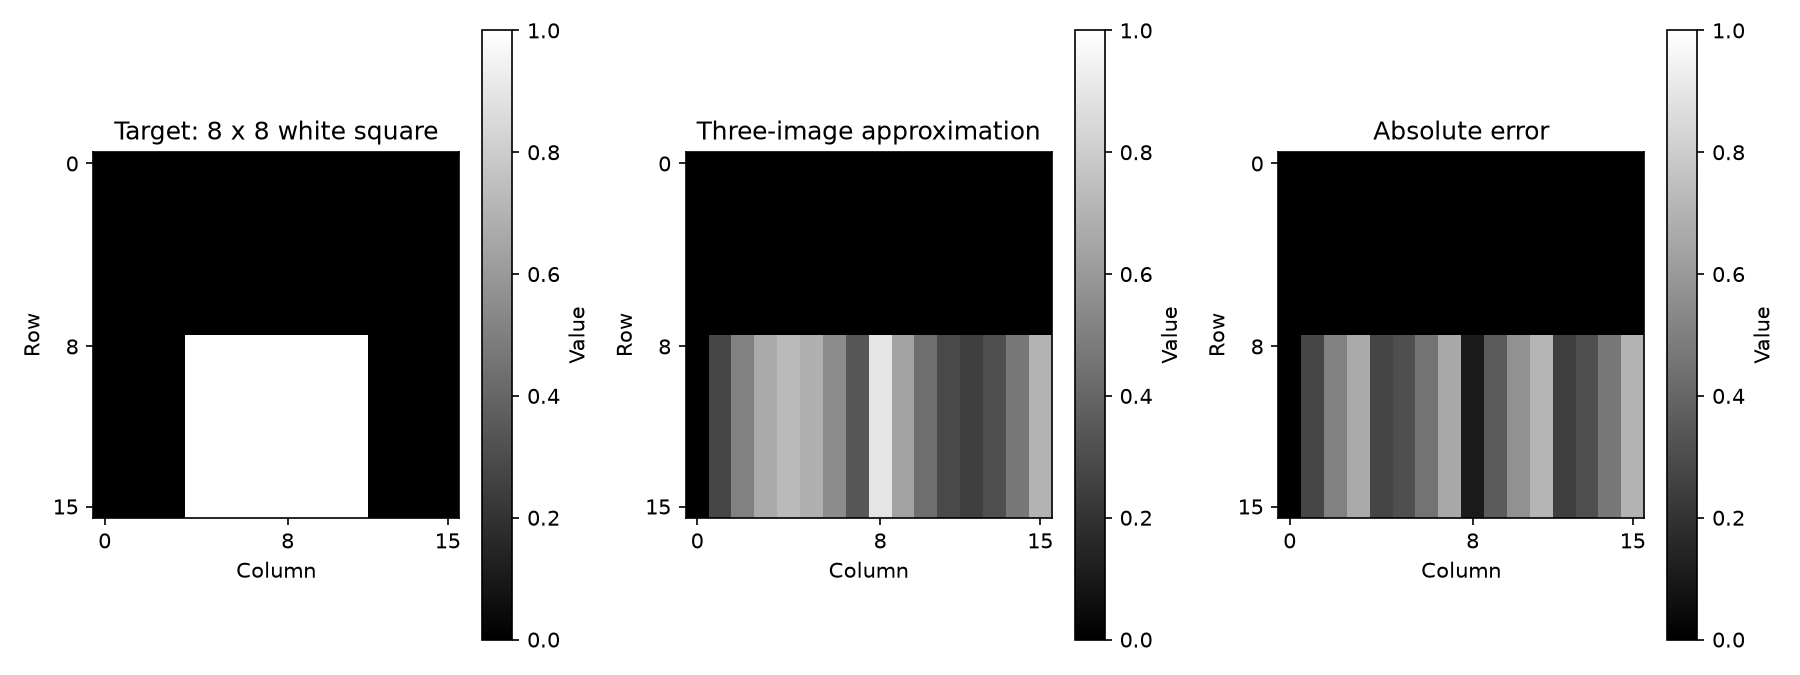
\includegraphics[trim=44.16bp 74.88bp 643.2bp 72.48bp,clip,width=\linewidth]{section7_shape_approximation.png}
\end{minipage}\hfill
\begin{minipage}{0.47\linewidth}\centering Three-image fit\\[2pt]
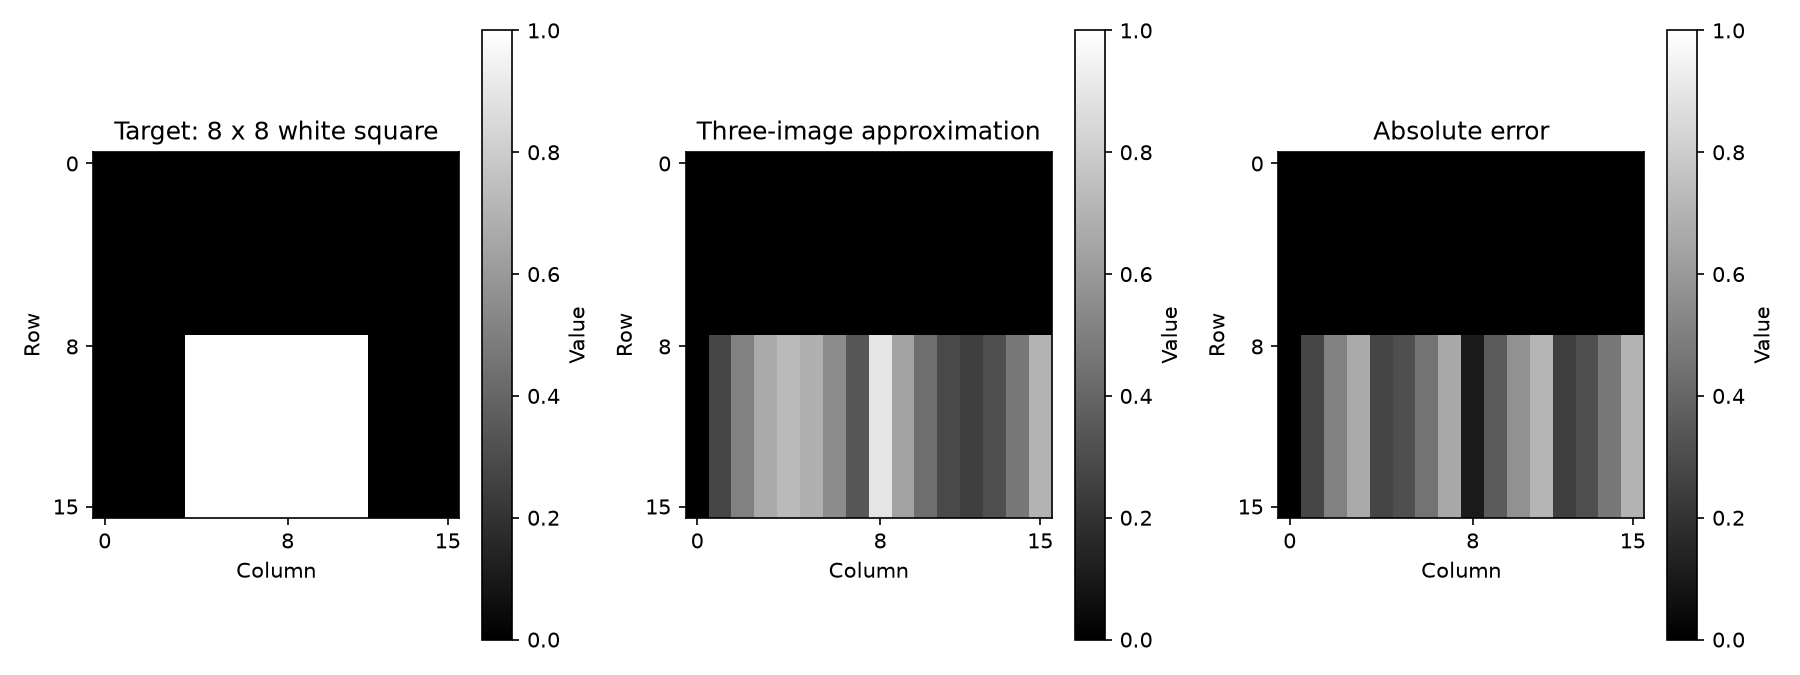
\includegraphics[trim=328.8bp 74.88bp 358.56bp 72.48bp,clip,width=\linewidth]{section7_shape_approximation.png}
\end{minipage}
\captionof{figure}{Q7.2: target and raw fit. Black 0 to white 1 in both.}\label{fig:shape}
\end{minipage}
\par

\subsection{Transforms and Frequency Domain}
\textbf{Q8.1.} The display used \texttt{log1p(abs(fftshift(fft2(gray))))}.
\texttt{fftshift} moves zero frequency (mean brightness) to the centre. The
actual spectrum has a bright central patch, with low frequencies nearby and
higher frequencies farther out. Horizontal/vertical streaks
are visible. Upright pepper sides plausibly contribute horizontal frequencies;
horizontal boundaries contribute vertical frequencies. Borders also contribute;
curved edges spread energy across directions. Magnitude shows frequency directions,
not spatial edge locations.

\textbf{Q8.2.} The circular low-pass kept radii below 40 bins in the \(512\times512\)
grid. Inverse shifting/FFT gave its real part. Main shapes stayed; detail weakened,
boundaries softened and the sharp cutoff caused ringing (Figure~\ref{fig:frequency}).
Raw range: \(-17.078\) to 243.781; negatives display black without changing data.

\textbf{Q8.3.} Floating-point original-minus-low-pass kept outlines, stems and detail,
with smooth areas near zero (Figure~\ref{fig:frequency}). Raw range:
\(-155.400\) to 113.396; display \(\pm155.400\), zero middle gray. Ringing remained.
Low-pass plus high-pass recovered the original with maximum error 0;
the inverse FFT's largest imaginary part was \(6.172\times10^{-14}\).

\begin{figure}[!htbp]\centering
\begin{minipage}[b]{0.31\linewidth}\centering Original\\[2pt]
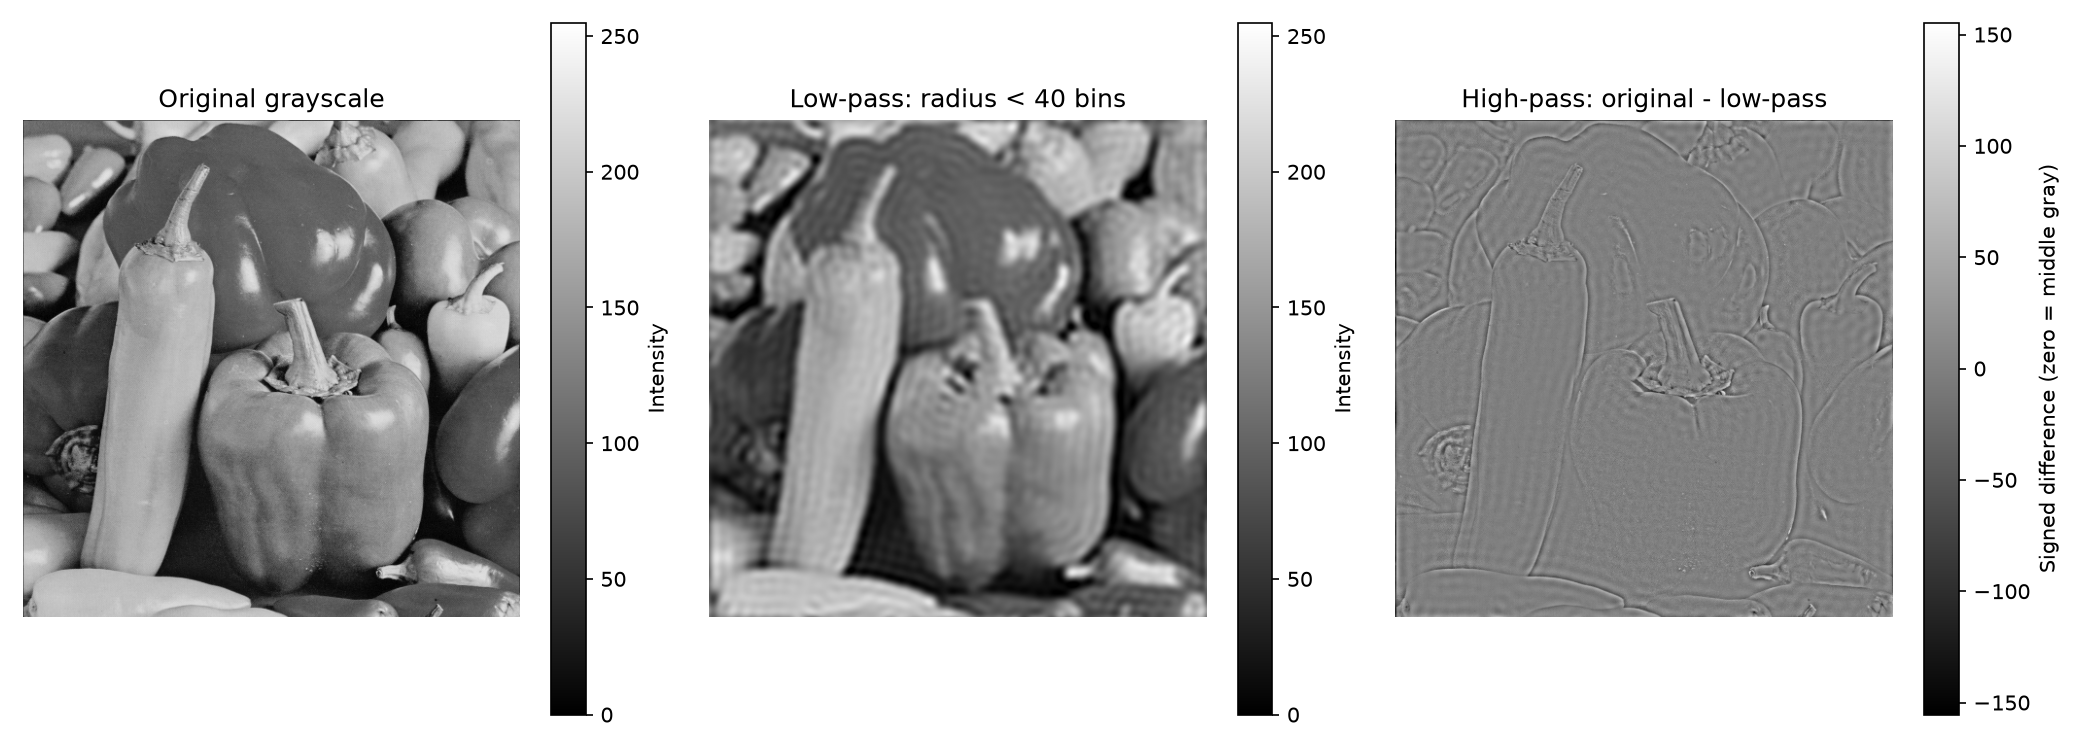
\includegraphics[trim=10.56bp 63.84bp 758.4bp 57.12bp,clip,width=\linewidth]{section8_frequency_filtering.png}
\end{minipage}\hfill
\begin{minipage}[b]{0.31\linewidth}\centering Low-pass\\[2pt]
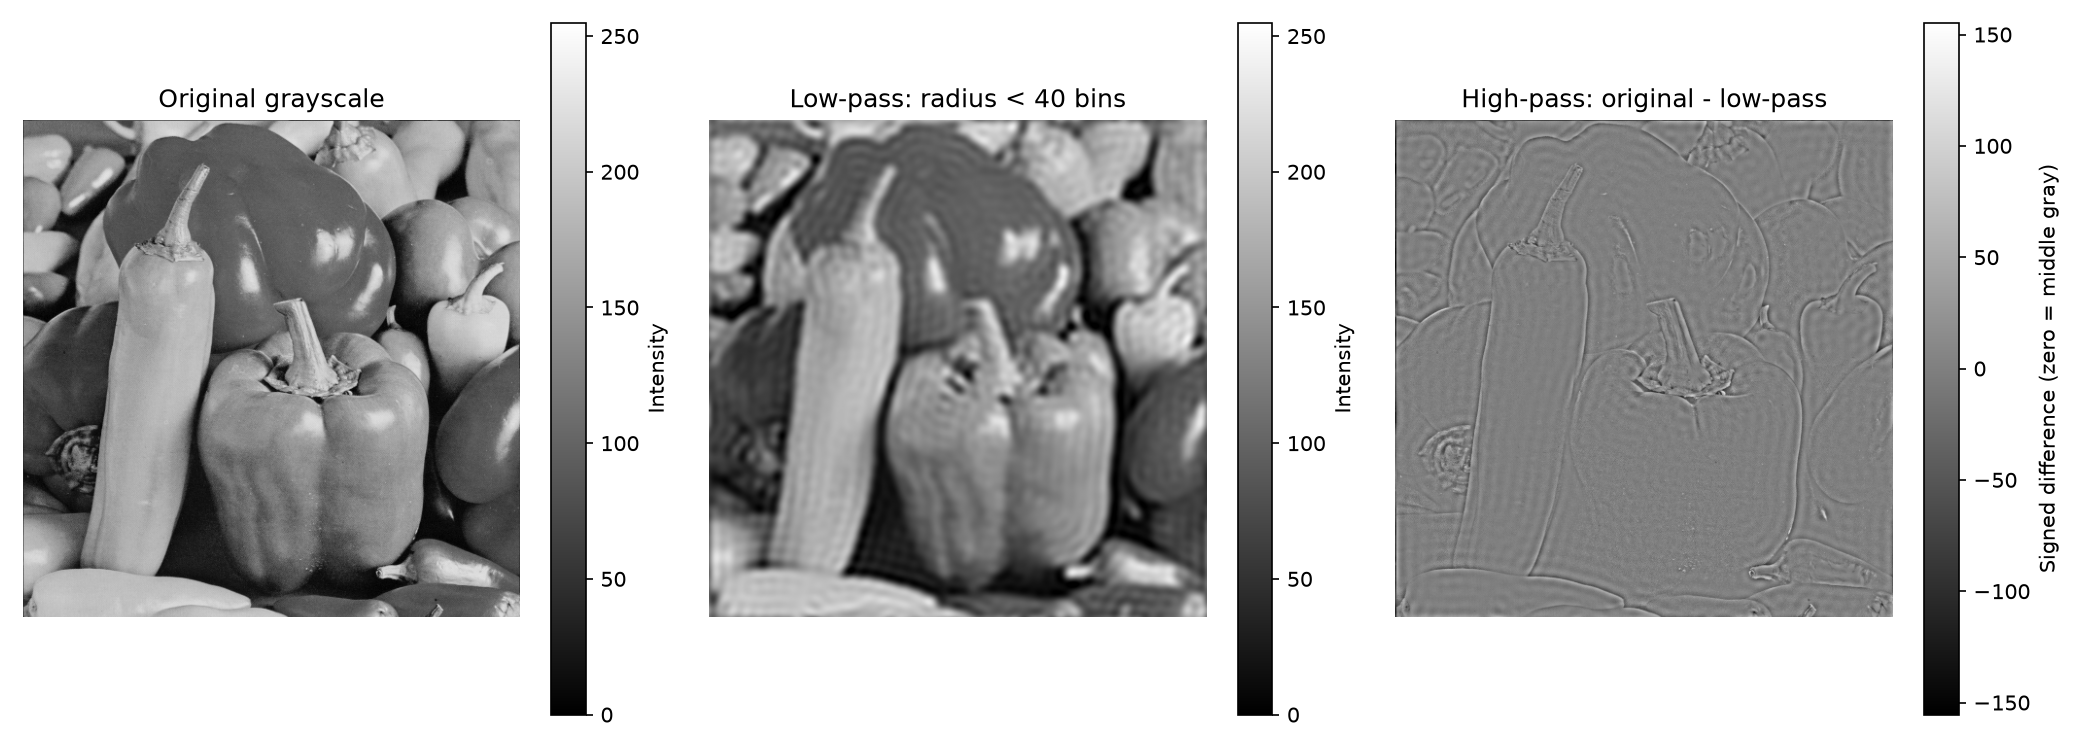
\includegraphics[trim=340.32bp 63.84bp 428.64bp 57.12bp,clip,width=\linewidth]{section8_frequency_filtering.png}
\end{minipage}\hfill
\begin{minipage}[b]{0.31\linewidth}\centering Signed high-pass\\[2pt]
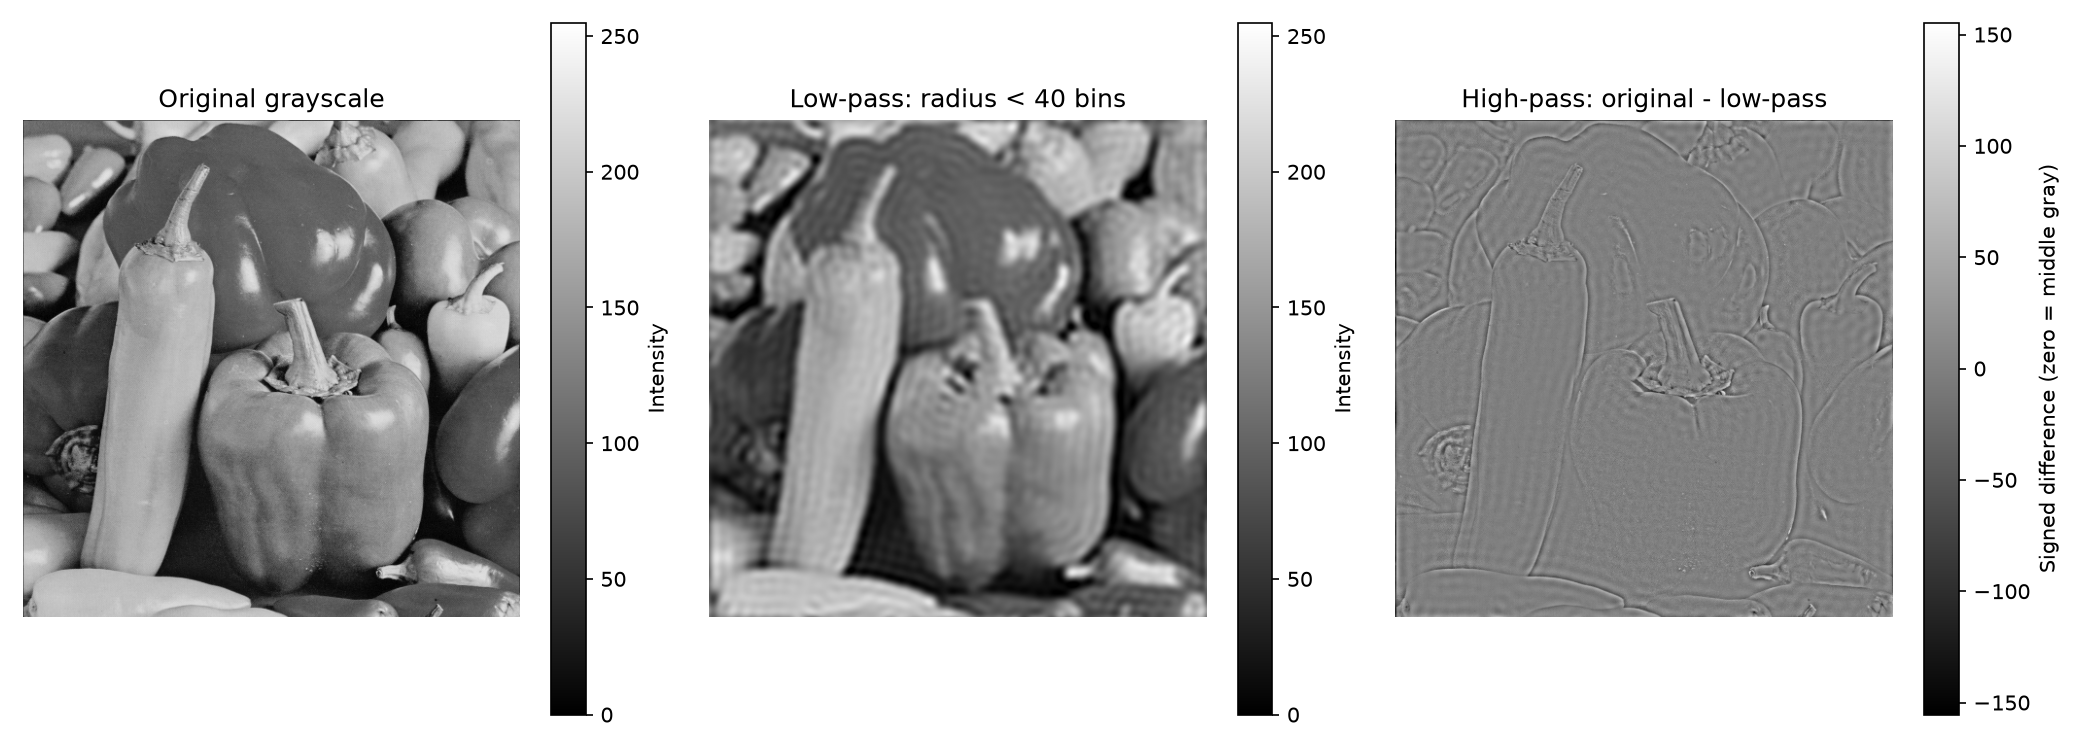
\includegraphics[trim=669.6bp 63.84bp 99.36bp 57.12bp,clip,width=\linewidth]{section8_frequency_filtering.png}
\end{minipage}
\caption{Q8.2--8.3: original/low-pass use 0--255; high-pass uses \(\pm155.400\), zero middle gray.}\label{fig:frequency}
\end{figure}

\subsection{Histograms and Image Enhancement}
\textbf{Q9.1.} The normalized histogram sums to 1 (Figure~\ref{fig:hist}): 76.43\% of
pixels were 64--191, the peak was 96, another group 150--190, maximum 228.
Cumulative values: 52.51\% at 127, 92.19\% at 191, reaching 1 at 228.
These show intensity amounts, not positions. \texttt{[0,256]} includes all levels
because OpenCV excludes the upper limit.



\begin{figure}[!htbp]\centering
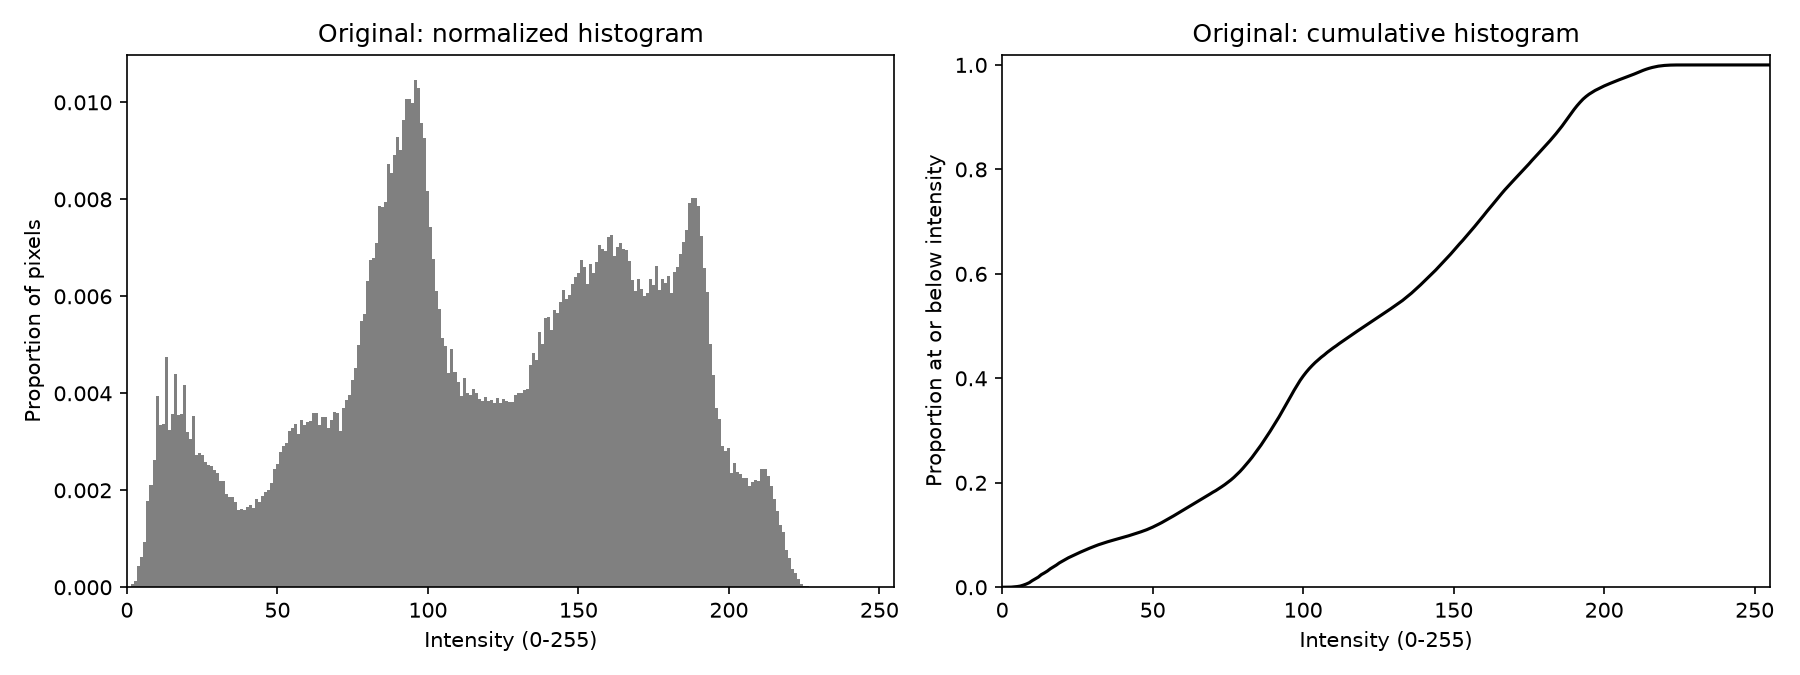
\includegraphics[width=160mm]{section9_histograms.png}
\caption{Q9.1: normalized histogram and cumulative histogram (CDF).}\label{fig:hist}
\end{figure}

\FloatBarrier
\begin{samepage}
\textbf{Q9.2.} Floating-point \(128+0.5(I-128)\) shrank 0--228 to 64--178.
\(T(r)=255\,\mathrm{CDF}(r)\), converted to \texttt{uint8}, restored 0--255;
OpenCV's \texttt{equalizeHist()} did too (Figure~\ref{fig:equalization}). Details
became clearer than the flat input; gaps/highlights were stronger than originally,
with more grain. Maximum difference: 1 level; mean: 0.443756. OpenCV subtracts
the first nonzero cumulative value and rounds; this method truncates the lab's formula.
\par\end{samepage}




\begin{figure}[H]\centering
\begin{minipage}[b]{0.235\linewidth}\centering Original\\[2pt]
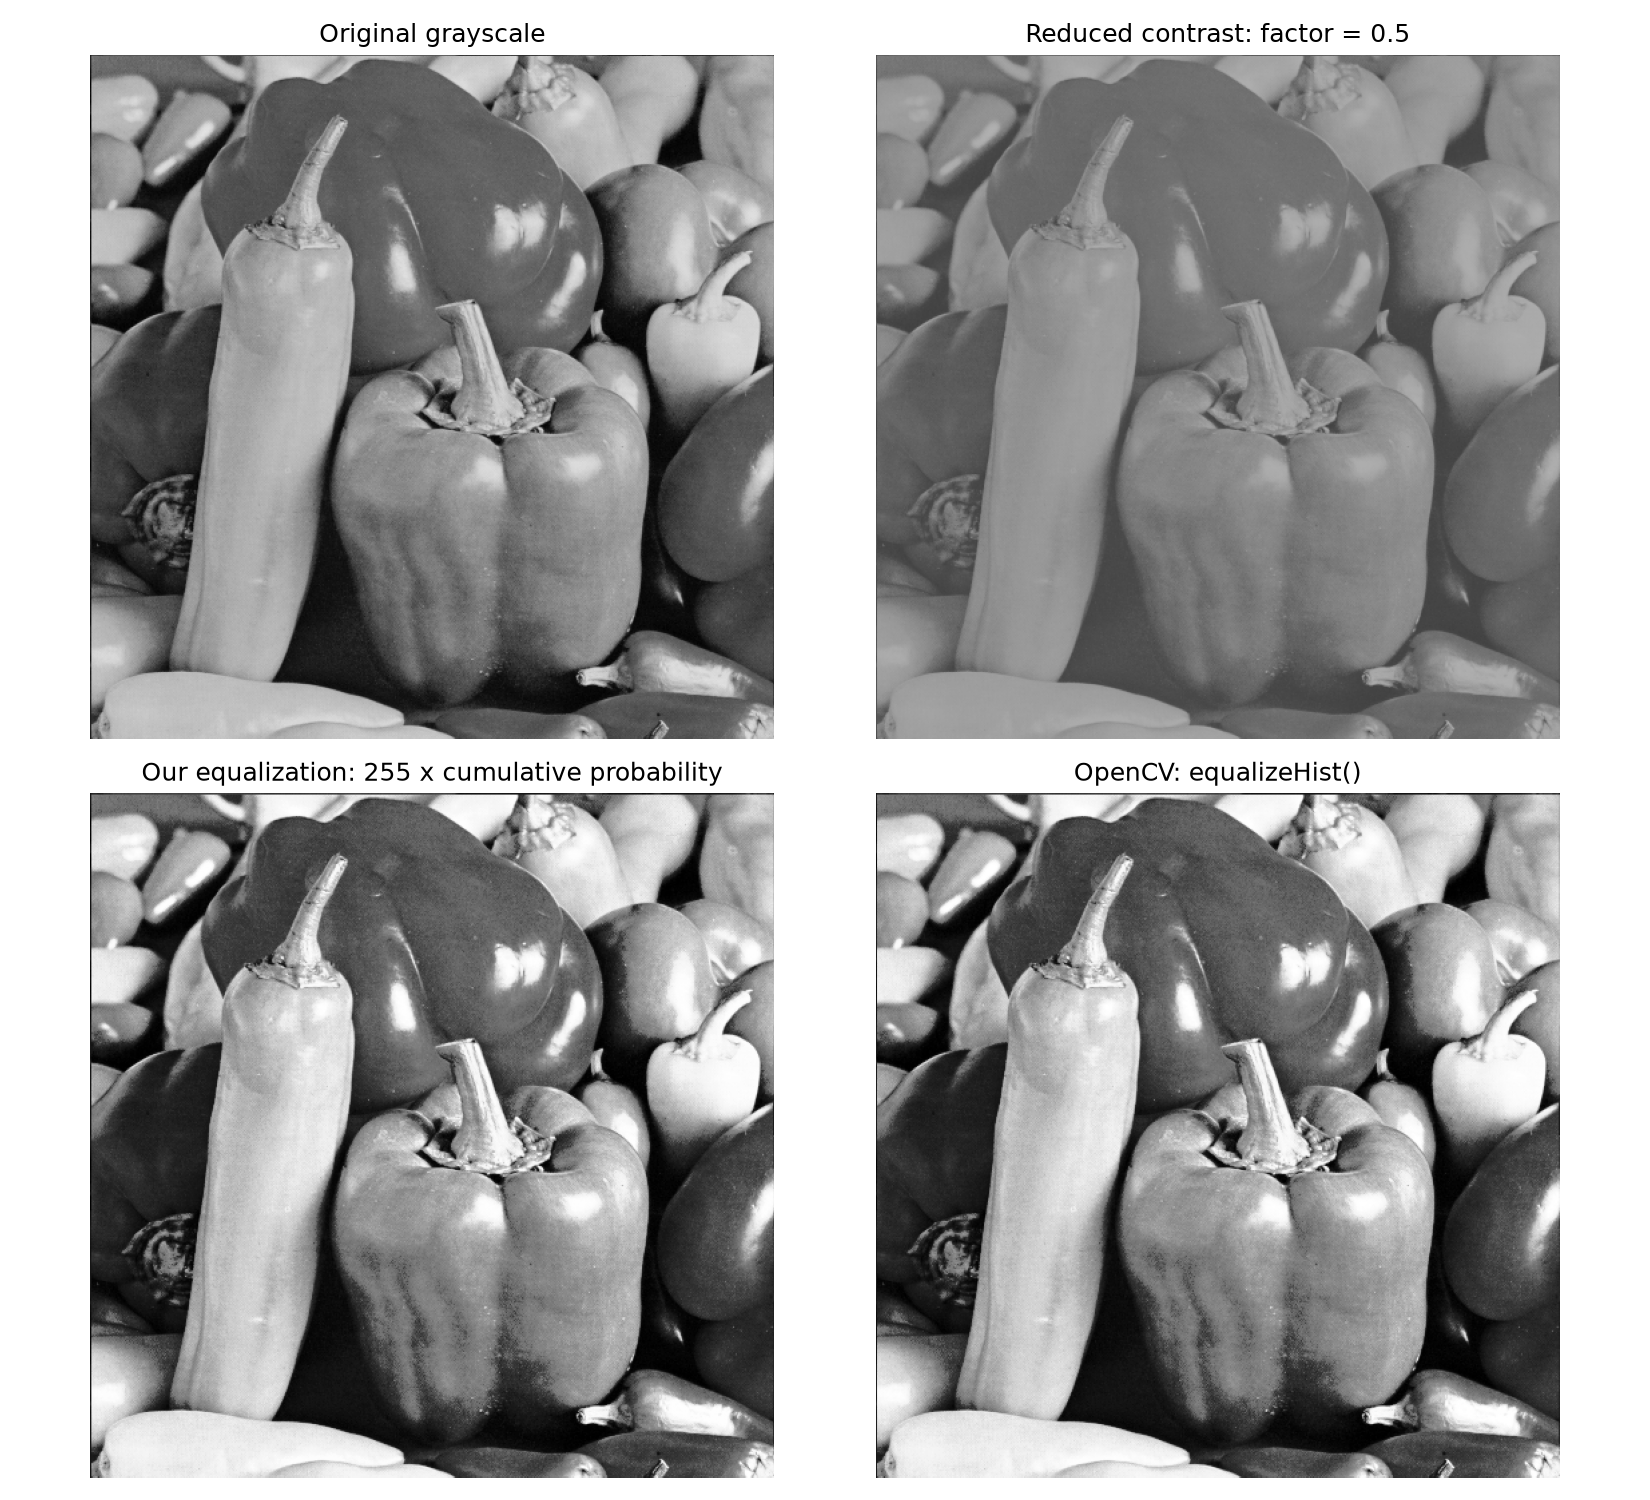
\includegraphics[trim=43.2bp 365.28bp 420.48bp 26.4bp,clip,width=\linewidth]{section9_histogram_equalization.png}
\end{minipage}\hfill
\begin{minipage}[b]{0.235\linewidth}\centering Contrast 0.5\\[2pt]
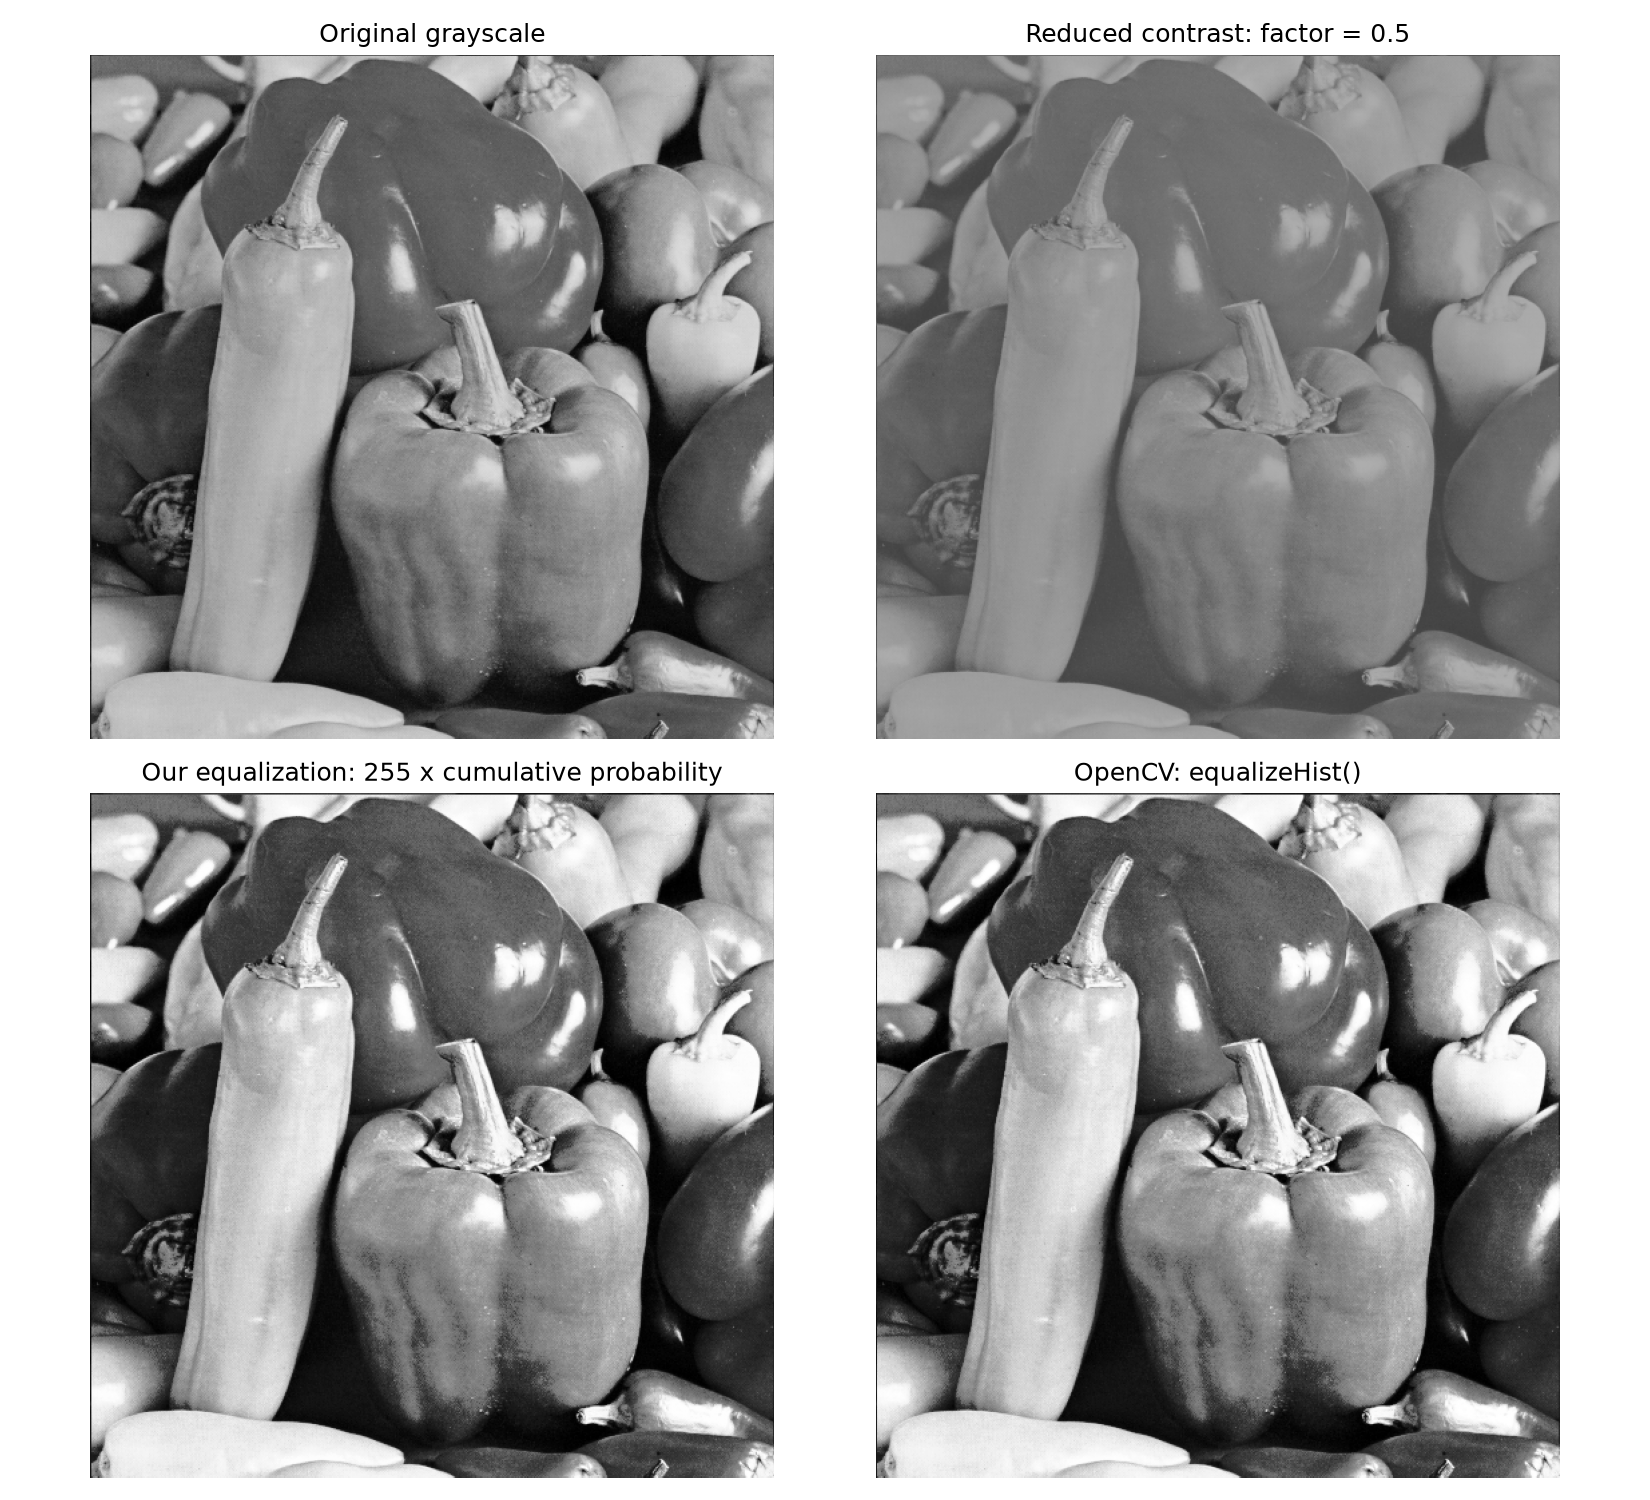
\includegraphics[trim=420.48bp 365.28bp 43.2bp 26.4bp,clip,width=\linewidth]{section9_histogram_equalization.png}
\end{minipage}\hfill
\begin{minipage}[b]{0.235\linewidth}\centering CDF method\\[2pt]
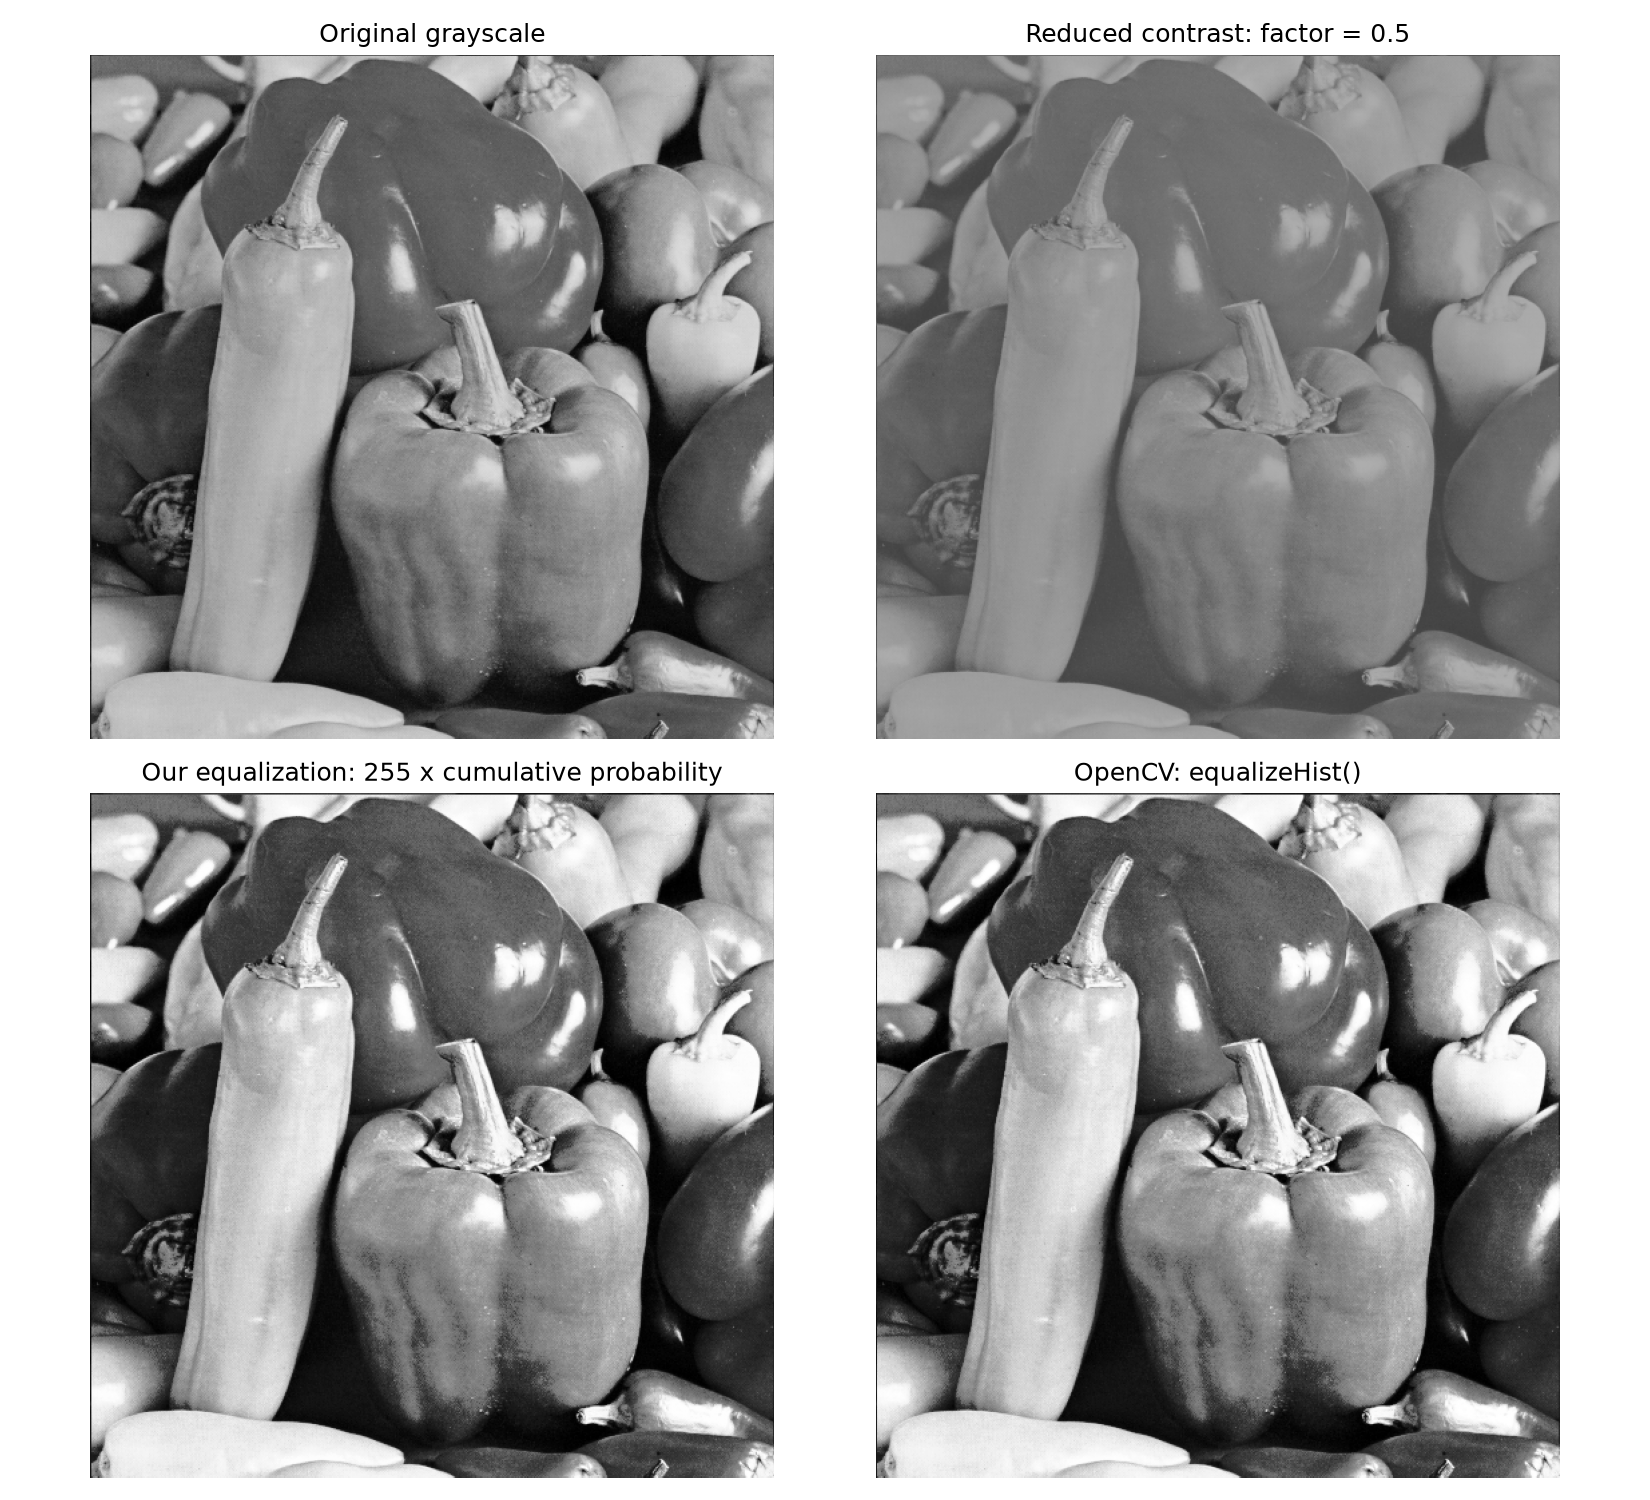
\includegraphics[trim=43.2bp 10.56bp 420.48bp 381.12bp,clip,width=\linewidth]{section9_histogram_equalization.png}
\end{minipage}\hfill
\begin{minipage}[b]{0.235\linewidth}\centering OpenCV\\[2pt]
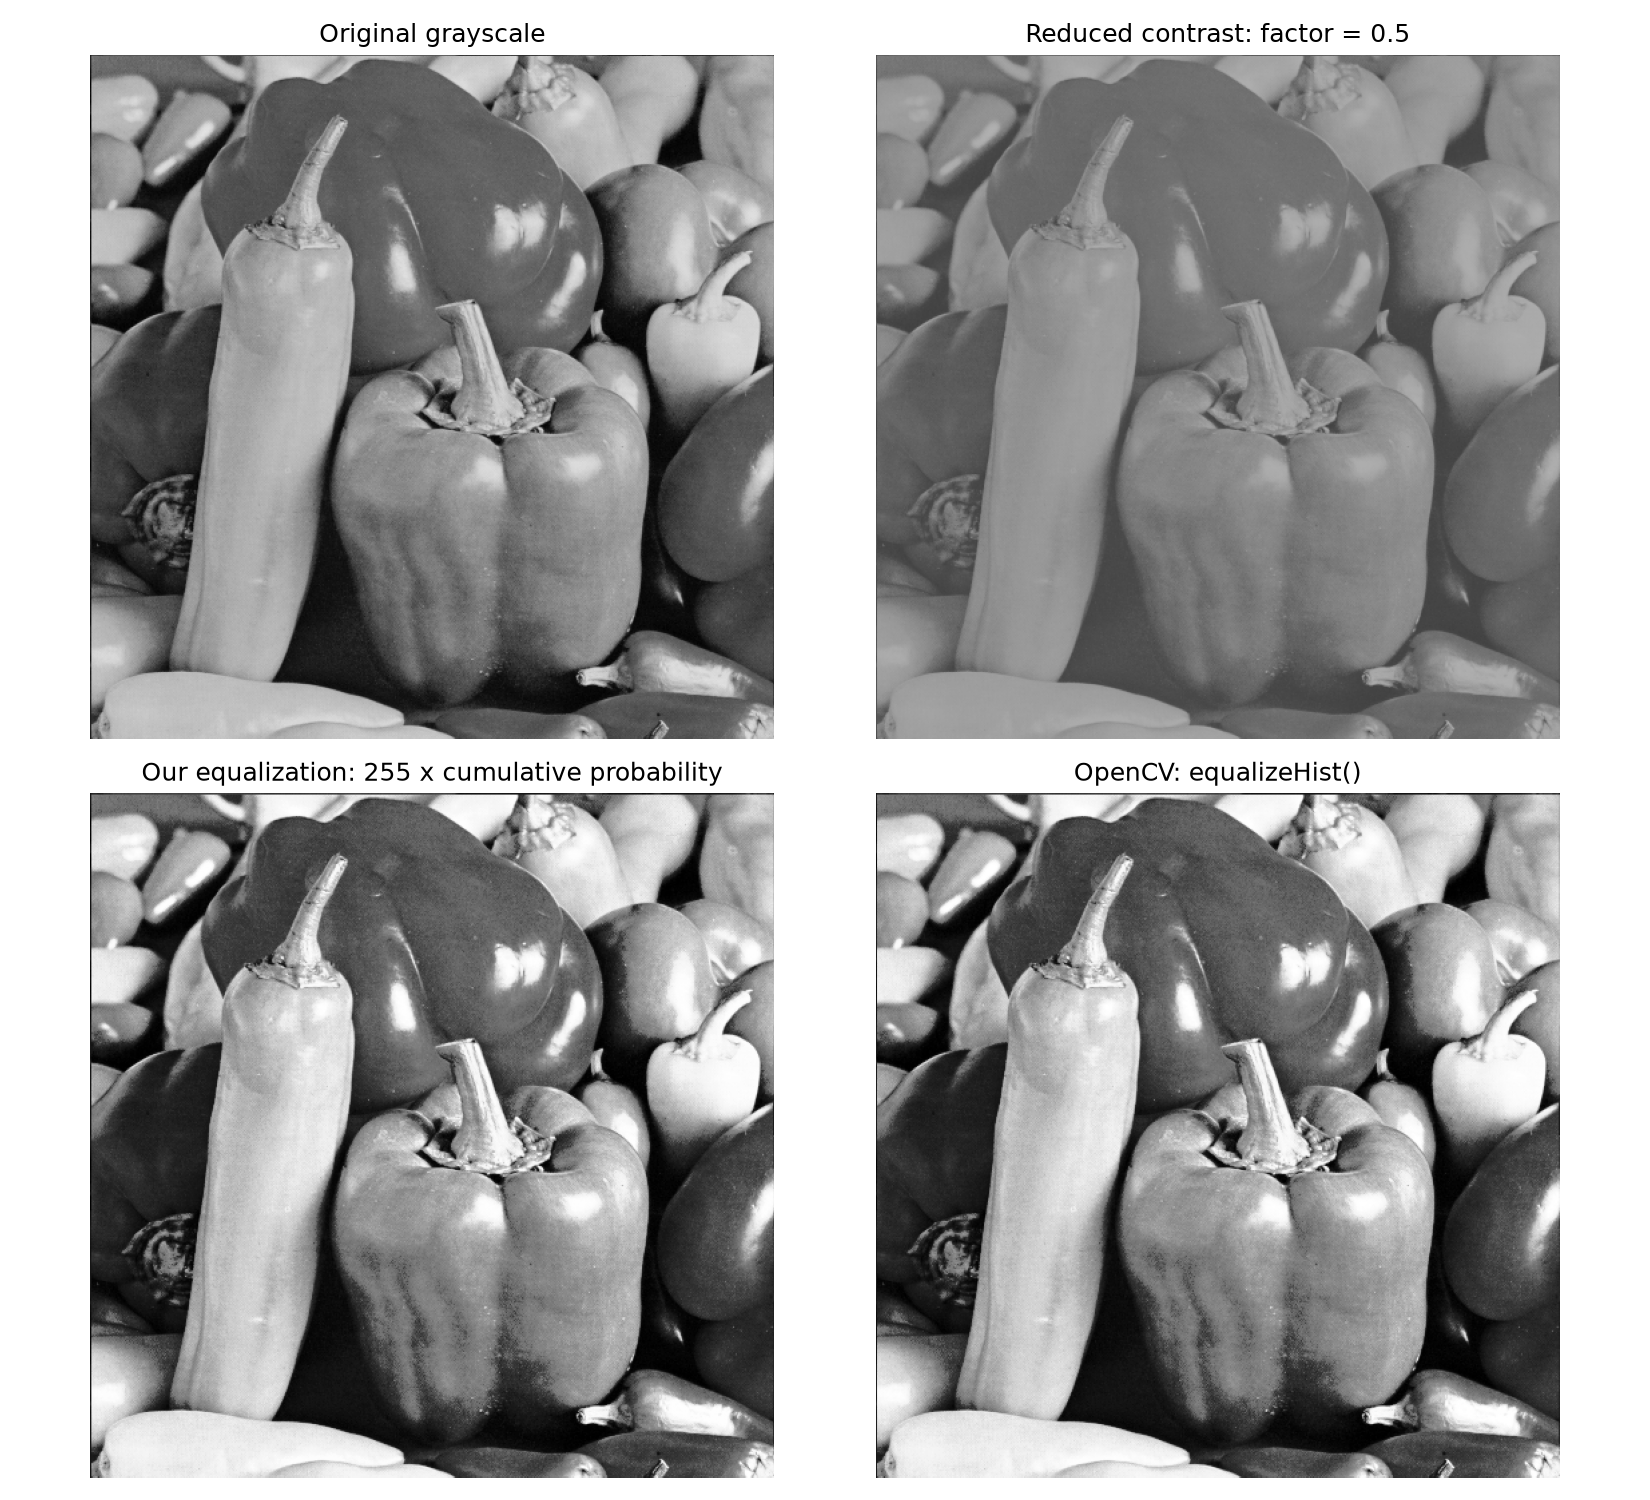
\includegraphics[trim=420.48bp 10.56bp 43.2bp 381.12bp,clip,width=\linewidth]{section9_histogram_equalization.png}
\end{minipage}
\caption{Q9.2: original, reduced contrast and two equalizations. All displays use 0--255.}\label{fig:equalization}
\end{figure}

\begin{samepage}
\subsection{Noise and Noise Reduction}
\textbf{Q10.1.} Seed 42 gave one zero-mean Gaussian sample, scaled and added as floats,
then clipped before integer conversion. Median \(3\times3\), noise \(\sigma=25\):
PSNR 20.318 to 26.829 dB. Bilateral (diameter 9, colour/spatial sigmas 75/75),
\(\sigma=35\): 17.519 to 26.888 dB.


The outputs approximately matched (0.059 dB gap), but different
input noise prevents same-input ranking. Bilateral trials \(\sigma=25,30,35\):
28.860, 28.004, 26.888 dB. Both reduced grain; bilateral was smoother but
softened stems. Similar PSNR did not mean identical appearance.
\par\end{samepage}

\begin{samepage}
\textbf{Q10.2.} Both \(3\times3\) filters received the same noisy input. PSNR in dB (input/mean/median; mean-minus-median): Gaussian \(\sigma=25\), 20.318/27.237/26.829 (\(+0.409\)); salt-and-pepper 4\%, 19.296/26.516/34.035 (\(-7.519\)). Salt-and-pepper probability was 4\% total: 2\% black,
2\% white, no overlap; 3.986\% selected. Mean gave slightly higher PSNR for Gaussian noise
but blurred edges. Median removed isolated extremes; mean spread them into gray
marks. \texttt{cv2.PSNR()} used the clean image; differences use unrounded values.
\par\end{samepage}



\subsection{Morphological Filtering}
\textbf{Q11.1.} Two \(128\times128\) binary tests used separated shapes: A had a circle,
rectangle and triangle; B added a different-size circle. Each had three white
specks and a \(2\times2\) hole. Opening with a \(3\times3\) cross removed specks;
closing with a \(5\times5\) ellipse filled holes. Eight-connected labels minus
background gave expected/detected 3/3 and 4/4. Corners rounded slightly;
touching objects would count together.

\begin{minipage}[t]{0.55\linewidth}\vspace{0pt}
\textbf{Q11.2.} Dilation minus erosion with the cross showed boundaries and more grain;
Sobel was smoother (Figure~\ref{fig:gradients}). Raw ranges 0--204 and 0--812.857
were separately normalized to 0--255: display brightness does not compare raw
strength. Morphology suits binary shapes and kernel-dependent boundaries;
Sobel suits grayscale changes and directional derivatives. Magnitude gives strength, not direction.
\end{minipage}\hfill
\begin{minipage}[t]{0.43\linewidth}\vspace{0pt}\centering
\begin{minipage}{0.47\linewidth}\centering Morphology\\[2pt]
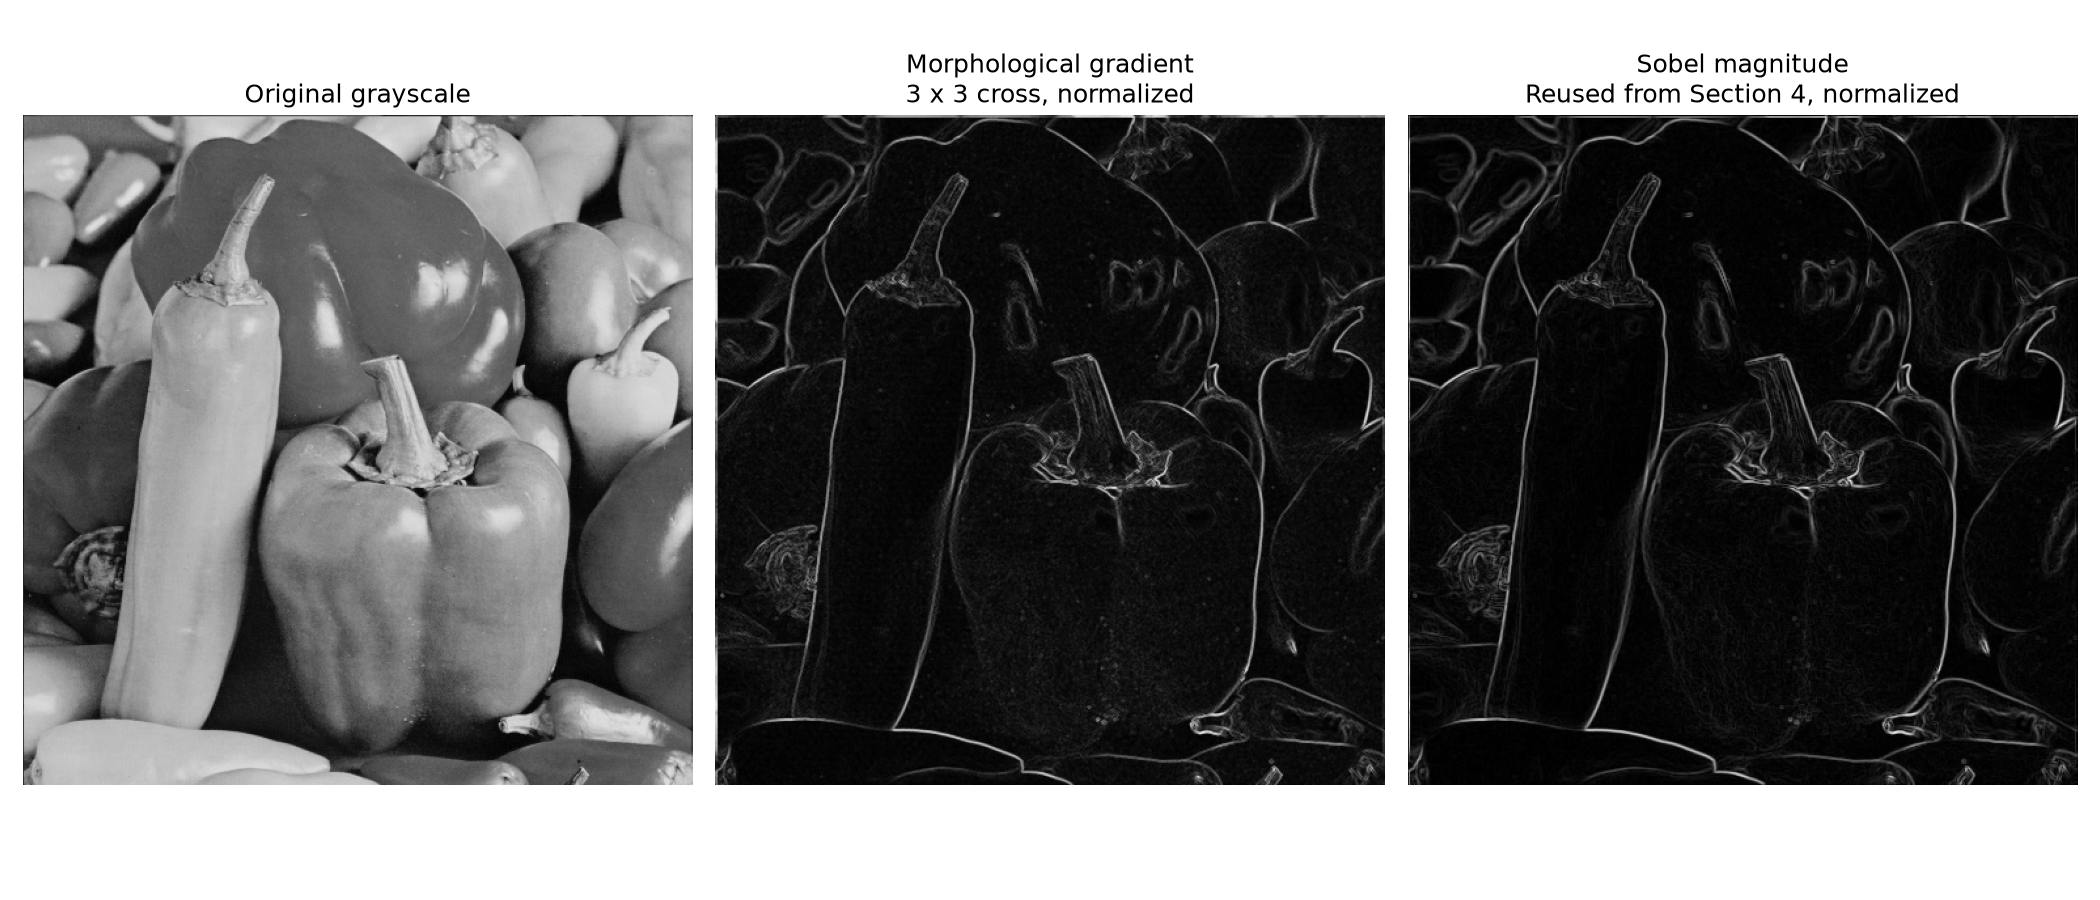
\includegraphics[trim=343.2bp 55.2bp 343.2bp 55.2bp,clip,width=\linewidth]{section11_gradient_comparison.png}
\end{minipage}\hfill
\begin{minipage}{0.47\linewidth}\centering Sobel\\[2pt]
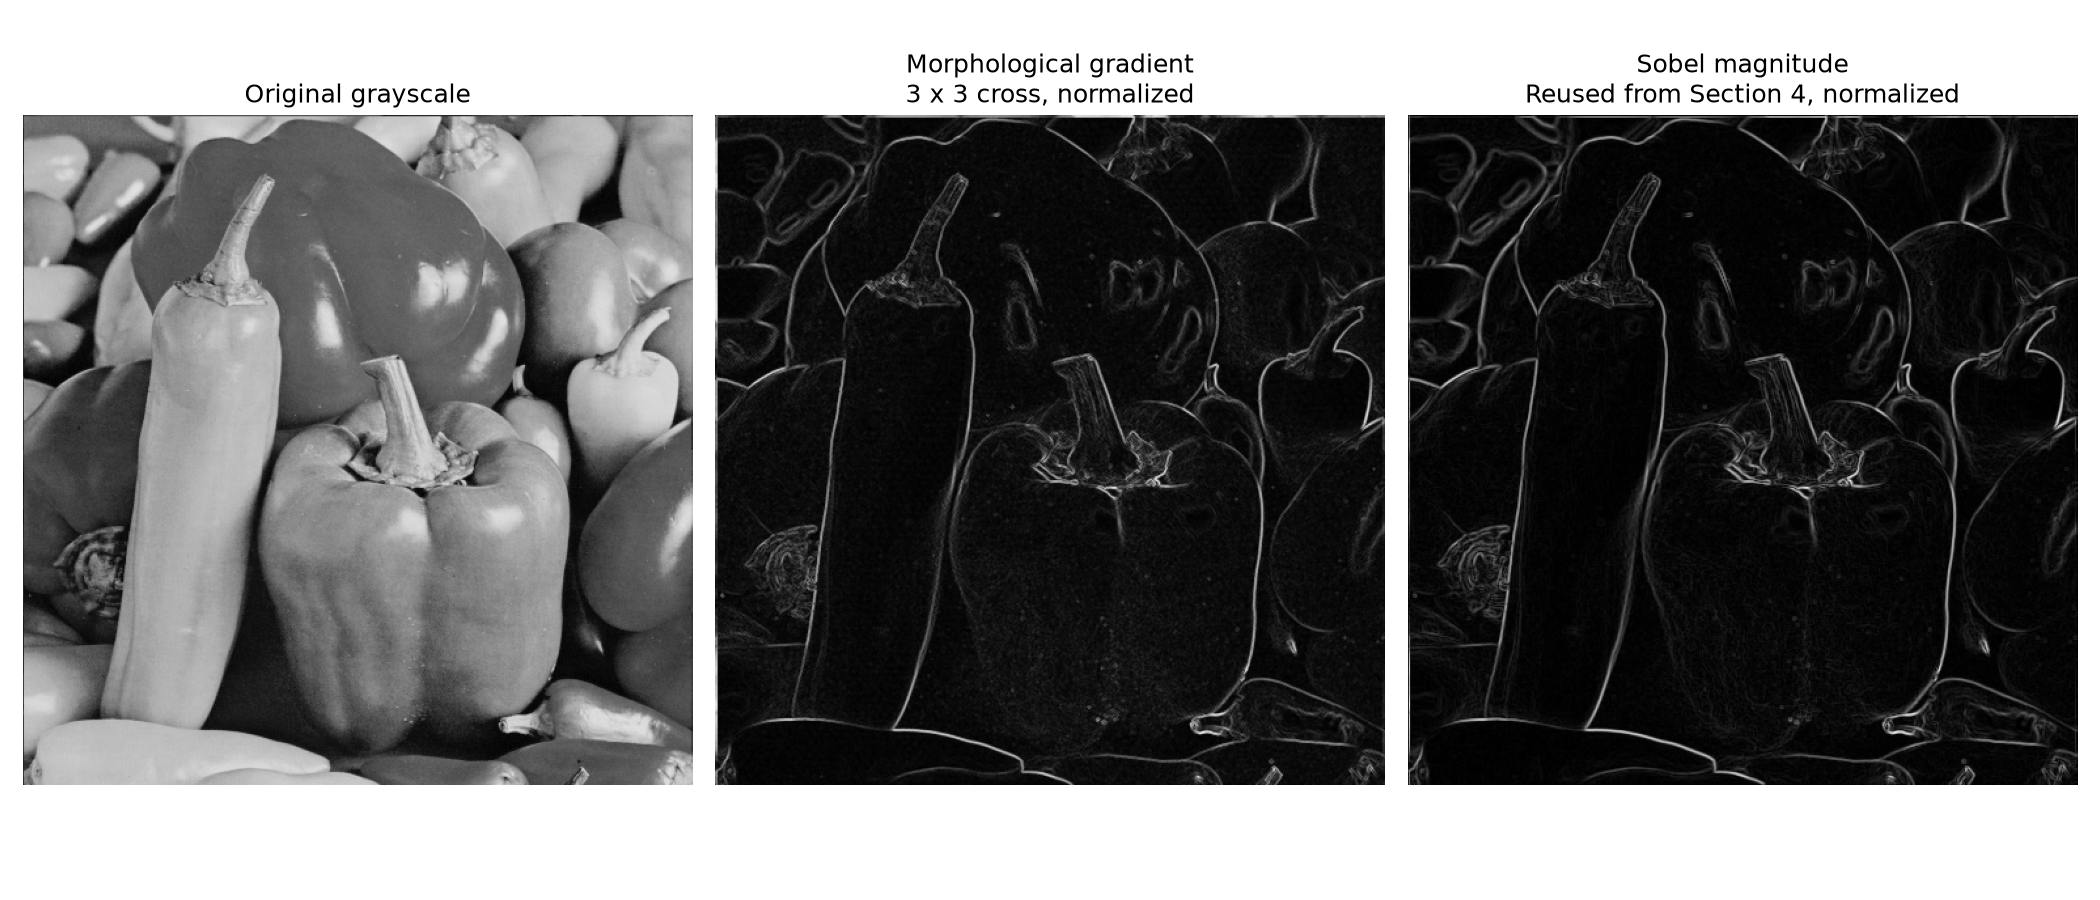
\includegraphics[trim=675.84bp 55.2bp 10.56bp 55.2bp,clip,width=\linewidth]{section11_gradient_comparison.png}
\end{minipage}
\captionof{figure}{Q11.2 and Q4.3: gradients, separately normalized to 0--255.}\label{fig:gradients}
\end{minipage}

\section{Discussion}
Vectorization and lookup saved time without changing outputs. Gaussian speed depended on routines; one run gives no general ranking. Filters traded noise against detail and depended on noise type. Equalization exposed grain. The coarse fit and touching-object limit show why settings and representation matter.

\section{Conclusion}
The experiments linked pixel values, colour, detail and frequency content.
Numerical results supported the image comparisons and explained time, memory
and noise trade-offs.

\section*{Appendix: Selected Implementation Code}
Excerpts from \texttt{lab3.py}, not standalone programs. NumPy is \texttt{np};
OpenCV is \texttt{cv2}; \texttt{gray} is the grayscale image.

\begin{minipage}[t]{0.49\linewidth}\vspace{0pt}\raggedright
\textbf{Q1.1: gamma.} Normalize, apply power, then \texttt{uint8}.
\lstinputlisting[linerange={11-11,13-15}]{../lab3.py}
\textbf{Q8.1--8.3: FFT filtering.} \texttt{lowpass\_mask} keeps radii below 40 bins from the centre.
\lstinputlisting[linerange={482-483,512-514,517-517}]{../lab3.py}
\end{minipage}\hfill
\begin{minipage}[t]{0.49\linewidth}\vspace{0pt}\raggedright
\textbf{Q4.2: horizontal Sobel.} Vertical derivative, \(3\times3\).
\lstinputlisting[firstline=256,lastline=258]{../lab3.py}
\textbf{Q11.1: object counting.} Inside the loop, \texttt{binary\_images[i]} is the test; kernels are the Q11.1 cross/ellipse.
\lstinputlisting[firstline=736,lastline=739,gobble=4]{../lab3.py}
\end{minipage}

\end{document}
